\documentclass[../Main.tex]{subfiles}
\usepackage{calc}
\usepackage{longtable}

\begin{document}
	\section{Proposed Research Model}
    This chapter presents a comprehensive research model designed to investigate the impact of university-based incubation programs (UBIs) on startup performance in Vietnam. The model posits that key components of incubation support influence startup success not only directly, but also indirectly by fostering a robust Entrepreneurial Orientation (EO) within the startup. The model is grounded in the \textbf{Resource-Based View (RBV)}, which emphasizes the role of unique resources and capabilities in achieving competitive advantage, and the \textbf{Technology-Organization-Environment (TOE)} framework, which considers the technological, organizational, and environmental factors affecting program impact.

    The proposed model, illustrating the relationships between the study's variables, is visually represented in the diagram below:
    \begin{figure}[H]
        \centering
        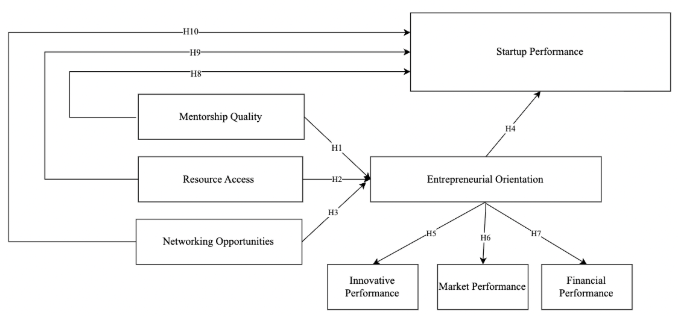
\includegraphics[width=\textwidth]{Figure/research_model.png}
        \caption{Proposed Research Model}
        \label{fig:research_model}
    \end{figure}

    The model is specifically tailored to Vietnam's developing entrepreneurial ecosystem, where startups face significant challenges such as limited funding, expertise, and market access. By examining the mediating role of EO, this research aims to provide a nuanced understanding of how UBIs create value, offering actionable insights for program optimization.

    \section{Variables of the Study}
    The research model is built upon a carefully selected set of variables designed to holistically capture the dynamics of university-based incubation in Vietnam. It comprises one dependent variable, three independent variables, one mediating variable, and four control variables, each grounded in established theory and adapted to the local context.
    \subsection{Dependent Variable}
    
    \textbf{Startup Performance}
    
    \textbf{Definition:} Startup Performance is conceptualized as a multidimensional construct that reflects the comprehensive success of a new venture. It moves beyond simple financial metrics to include innovative achievements and market traction. Specifically, it encompasses:
    
    \begin{itemize}
        \item \textbf{Innovative Performance:} The startup's ability to develop and launch new products, services, or internal processes.
        \item \textbf{Market Performance:} The startup's success in growing its market share, acquiring new customers, and increasing sales.
        \item \textbf{Financial Performance:} The startup's financial health, measured by revenue growth, profitability, and return on investment.
    \end{itemize}
    
    \textbf{Theoretical Grounding:} This variable is supported by two key frameworks. The Resource-Based View (RBV) posits that superior performance is a direct result of the effective deployment of valuable resources and capabilities, such as those provided by an incubator. The Technology-Organization-Environment (TOE) framework contextualizes this performance by considering the interplay of technological factors (e.g., innovation tools), organizational strategies, and environmental conditions (e.g., market dynamics).
    
    \textbf{Measurement:} A mixed-method approach will be used to measure Startup Performance robustly:
    
    \begin{itemize}
        \item \textbf{Quantitative Metrics:} Objective data will be collected from official records, including the number of new products launched or patents filed (Innovative), percentage increase in market share or customer acquisition rates (Market), and year-on-year revenue growth or profit margins (Financial).
        \item \textbf{Qualitative Data:} Founders' subjective perceptions will be captured through a 5-point Likert scale (1 = strongly disagree, 5 = strongly agree) with targeted questions such as, ``Our market share has increased due to incubator support'' and ``Our financial performance has improved due to incubator support''. This combination of objective and subjective data ensures a comprehensive and reliable measurement.
    \end{itemize}
    
    \textbf{Relevance to Vietnam:} For Vietnamese startups, which often operate with limited capital, constrained technological access, and difficulties in market penetration, achieving strong performance across these three dimensions is a critical indicator of success and sustainability. This variable directly measures the effectiveness of UBIs in helping startups overcome these specific local challenges.

    \subsection{Independent Variables}
    
    The independent variables represent the core components of support that university-based incubation programs provide.
    
    \textbf{1. Mentorship Quality}
    
    \textbf{Definition:} Refers to the caliber, accessibility, and effectiveness of the guidance provided by mentors within the UBI. This involves tailored advice on business strategy, technical development, market entry, and operational management from mentors with relevant industry or entrepreneurial experience.
    
    \textbf{Theoretical Grounding:} From an RBV perspective, high-quality mentorship is a valuable human resource that builds a startup's knowledge-based capabilities. The TOE framework positions mentorship as a critical organizational factor that facilitates the effective adoption of other forms of incubation support.
    
    \textbf{Measurement:} Mentorship Quality will be assessed using:
    \begin{itemize}
        \item \textbf{Quantitative Metrics:} Number of mentorship sessions per month, mentor qualifications (e.g., years of industry experience, academic credentials), and mentor-to-startup ratio, collected from incubator records.
        \item \textbf{Qualitative Data:} A 5-point Likert scale survey will measure founders' perceptions of mentor expertise, responsiveness, and impact, using items adapted from validated scales (e.g., ``Mentors provided actionable advice for strategic growth'').
    \end{itemize}
    
    \textbf{Relevance to Vietnam:} In Vietnam's nascent entrepreneurial ecosystem, there is a significant lack of experienced business leaders. UBIs fill this critical gap by leveraging academic faculty and industry alumni, providing the strategic decision-making support that local startups desperately need.
    
    \textbf{2. Resource Access}
    
    \textbf{Definition:} Encompasses the tangible and intangible resources that an incubator provides, including seed funding, office space, technology infrastructure (e.g., software, cloud services), and privileged access to university research facilities like labs and libraries.
    
    \textbf{Theoretical Grounding:} RBV considers these resources as fundamental assets for building a competitive advantage. Within the TOE framework, Resource Access is a key technological factor that directly enables innovation and operational efficiency.
    
    \textbf{Measurement:} Resource Access will be measured through:
    \begin{itemize}
        \item \textbf{Quantitative Metrics:} Amount of seed funding provided (in USD equivalent), hours of access to research facilities, and square footage of office space, sourced from incubator financial reports and resource logs.
        \item \textbf{Qualitative Data:} A 5-point Likert scale survey will capture founders' perceptions of resource adequacy and its impact on their operations (e.g., ``Access to university resources enabled product development'').
    \end{itemize}
    
    \textbf{Relevance to Vietnam:} Access to capital and technology remains a major barrier for most Vietnamese startups. UBIs, often backed by government initiatives, are uniquely positioned to provide these foundational resources, making this variable a critical determinant of startup growth in the country.
    
    \textbf{3. Networking Opportunities}
    
    \textbf{Definition:} Refers to the incubator's role in facilitating valuable connections for startups, including introductions to investors, potential industry partners, and a community of peer entrepreneurs. These networks are vital for securing funding, building strategic partnerships, and gaining market access.
    
    \textbf{Theoretical Grounding:} RBV views networks as valuable relational resources that provide a distinct competitive advantage. The TOE framework positions networking as an environmental factor that shapes a startup's trajectory through external linkages.
    
    \textbf{Measurement:} This variable will be assessed via:
    \begin{itemize}
        \item \textbf{Quantitative Metrics:} Number of networking events attended, investor introductions made by the incubator, and formal partnerships formed as a result of these connections, collected from incubator logs.
        \item \textbf{Qualitative Data:} A 5-point Likert scale survey will measure founders' perceptions of the quality and value of networking support (e.g., ``Networking through the incubator led to valuable partnerships'').
    \end{itemize}
    
    \textbf{Relevance to Vietnam:} The entrepreneurial ecosystem in Vietnam often lacks robust, well-established industry networks. UBIs play a crucial role in bridging this gap, connecting startups to investors, alumni, and industry leaders, thereby enhancing their market opportunities in a way they could not achieve alone.

    \subsection{Mediating Variable}
    
    \textbf{Entrepreneurial Orientation (EO)}
    
    \textbf{Definition:} Entrepreneurial Orientation is a firm-level strategic posture reflecting a company's willingness to engage in innovative, proactive, and risk-taking behaviors. It is not an outcome itself, but a mindset and a set of processes that enables startups to effectively leverage the support they receive and convert it into performance. It consists of three dimensions:
    \begin{itemize}
        \item \textbf{Innovativeness:} The tendency to pursue new ideas and solutions.
        \item \textbf{Proactiveness:} The forward-looking ability to anticipate and act on future market opportunities.
        \item \textbf{Risk-Taking:} The willingness to commit resources to projects with uncertain outcomes.
    \end{itemize}
    
    \textbf{Theoretical Grounding:} From an RBV perspective, EO is considered a dynamic capability that allows a firm to integrate, build, and reconfigure internal and external competences to address rapidly changing environments. Within the TOE framework, EO is an organizational factor that enhances the firm's ability to absorb and benefit from technological and environmental opportunities.
    
    \textbf{Measurement:} EO will be measured using:
    \begin{itemize}
        \item \textbf{Quantitative Metrics:} Number of new initiatives launched (innovativeness), time-to-market for new products (proactiveness), and investment in high-risk projects (risk-taking).
        \item \textbf{Qualitative Data:} Founders' self-reported EO will be measured using a 5-point Likert scale survey based on validated scales (e.g., Covin \& Slevin, 1989), with items like ``Our startup actively pursues innovative solutions'' and ``We take bold actions to enter new markets''.
    \end{itemize}
    
    \textbf{Relevance to Vietnam:} In the highly competitive and rapidly evolving Vietnamese market, a strong EO is essential for survival and growth. It is the critical mechanism through which incubator support is transformed into tangible innovation and market success.

    \subsection{Control Variables}
    
    To ensure the validity of the findings by accounting for extraneous factors, the following control variables are included:
    
    \begin{itemize}
        \item \textbf{Startup Age:} Measured in years since founding, as younger startups may be more dependent on incubator support and have different performance trajectories than more mature ones.
        \item \textbf{Industry Sector:} Categorized into key sectors like technology, fintech, or retail, because incubation needs and performance benchmarks vary significantly across industries.
        \item \textbf{Founder Experience:} Measured by the founder's total years of entrepreneurial or relevant industry experience, as this can heavily influence their ability to utilize program resources effectively.
        \item \textbf{University Type:} Coded as either public or private, as the availability of resources and the underlying mission of the incubator may differ between these institutional types.
    \end{itemize}

    \section{Hypothesis Development}
    The following hypotheses are formulated to empirically test the relationships proposed in the research model.

    \subsection{Hypothesis 1 (H1)}
    \textbf{Hypothesis:} Mentorship Quality is positively related to Entrepreneurial Orientation.
    
    \textbf{Theoretical Foundation:} This hypothesis is grounded in the Resource-Based View (RBV) theory \cite{barney1991firm}, which posits that human capital resources, particularly knowledge and expertise, are fundamental to building competitive advantages. The relationship is also supported by Social Learning Theory \cite{bandura1997self}, which suggests that entrepreneurs learn strategic behaviors through observation and interaction with experienced mentors.
    
    \textbf{Relationship:} This hypothesis suggests that as the quality of mentorship provided by a UBI increases, the startup's strategic orientation toward innovativeness, proactiveness, and risk-taking will be strengthened. The relationship operates through multiple mechanisms: knowledge transfer, confidence building, and strategic mindset development.
    
    \textbf{Rationale:} High-quality mentors provide founders with specialized knowledge, practical experience, and strategic direction that directly influence their entrepreneurial mindset. This guidance empowers founders in three critical ways:
    \begin{itemize}
        \item \textbf{Knowledge Enhancement:} Mentors share industry insights, market trends, and technical expertise that enable founders to make informed decisions about innovation opportunities.
        \item \textbf{Confidence Building:} Through regular interaction and validation, mentors help founders develop the confidence to experiment with new ideas (innovativeness), anticipate and act on market opportunities (proactiveness), and make calculated, bold decisions (risk-taking).
        \item \textbf{Strategic Perspective:} Mentors provide a broader strategic perspective that helps founders understand the long-term implications of their decisions and encourages forward-thinking behavior.
    \end{itemize}
    
    \textbf{Contextual Relevance:} In Vietnam's nascent entrepreneurial ecosystem, where many young founders lack managerial and strategic experience, guidance from seasoned mentors is invaluable \cite{dinh2017promoting}. The country's educational system has traditionally emphasized technical skills over entrepreneurial thinking, creating a significant "knowledge gap" that UBIs help bridge. Mentors in Vietnamese UBIs often include successful alumni, industry experts, and international entrepreneurs who bring diverse perspectives and global best practices.
    
    \textbf{Empirical Support:} Previous research has demonstrated that mentorship quality is positively associated with entrepreneurial self-efficacy and intention \cite{bandura1997self, zhao2005developing}. Studies in emerging markets have shown that mentor guidance significantly influences startup strategic orientation \cite{sullivan2011effectiveness}.
    
    \textbf{Supporting Variables:}
    \begin{itemize}
        \item Independent Variable: Mentorship Quality (measured through mentor qualifications, session frequency, and founder satisfaction).
        \item Dependent Variable: Entrepreneurial Orientation (measured through innovativeness, proactiveness, and risk-taking dimensions).
    \end{itemize}

    \subsection{Hypothesis 2 (H2)}
    \textbf{Hypothesis:} Resource Access is positively related to Entrepreneurial Orientation.
    
    \textbf{Theoretical Foundation:} This hypothesis is supported by the Resource-Based View (RBV) theory \cite{barney1991firm}, which emphasizes that access to valuable, rare, and inimitable resources creates competitive advantages. The relationship is also grounded in Resource Dependency Theory \cite{pfeffer1978external}, which suggests that organizations' strategic behaviors are shaped by their access to critical resources.
    
    \textbf{Relationship:} This hypothesis posits that greater access to essential resources (capital, technology, facilities, and infrastructure) will foster a stronger Entrepreneurial Orientation. The relationship operates through resource slack theory \cite{cyert1963behavioral}, which suggests that having access to resources beyond immediate needs enables organizations to pursue innovative and proactive strategies.
    
    \textbf{Rationale:} When basic resource constraints are alleviated, startups have the "breathing room" to be creative and take risks. This relationship manifests through several mechanisms:
    \begin{itemize}
        \item \textbf{Financial Slack:} Access to seed funding and financial resources allows startups to invest in R\&D, experimental projects, and long-term initiatives without immediate pressure for returns, fostering innovativeness and risk-taking.
        \item \textbf{Technological Capabilities:} Access to advanced technology infrastructure, software, and research facilities enables startups to develop cutting-edge solutions and stay ahead of competitors, enhancing their proactive stance.
        \item \textbf{Operational Flexibility:} Access to office space, equipment, and support services reduces operational burdens, allowing founders to focus on strategic thinking and innovation rather than day-to-day survival.
        \item \textbf{Knowledge Resources:} Access to university libraries, databases, and research networks provides startups with the information needed to make informed strategic decisions and identify new opportunities.
    \end{itemize}
    
    \textbf{Contextual Relevance:} The lack of capital and technology remains a primary obstacle for most Vietnamese startups \cite{vietnam_innovation_report_2024}. According to recent surveys, over 60\% of Vietnamese startups cite funding as their biggest challenge, while 45\% struggle with access to technology and infrastructure. UBIs, often backed by government initiatives and university resources, are uniquely positioned to provide these foundational resources, creating a crucial safety net that enables startups to pursue innovative and proactive strategies more aggressively.
    
    \textbf{Empirical Support:} Research has consistently shown that resource availability is positively associated with entrepreneurial orientation \cite{wiklund2005entrepreneurial}. Studies in emerging markets have demonstrated that access to financial and technological resources significantly influences startup strategic behavior \cite{bruton2010governance}.
    
    \textbf{Supporting Variables:}
    \begin{itemize}
        \item Independent Variable: Resource Access (measured through funding amount, facility access hours, and technology infrastructure availability).
        \item Dependent Variable: Entrepreneurial Orientation (measured through innovativeness, proactiveness, and risk-taking dimensions).
    \end{itemize}

    \subsection{Hypothesis 3 (H3)}
    \textbf{Hypothesis:} Networking Opportunities are positively related to Entrepreneurial Orientation.
    
    \textbf{Theoretical Foundation:} This hypothesis is grounded in Social Network Theory \cite{granovetter1973strength}, which posits that an organization's position within a network of relationships provides access to valuable information, resources, and opportunities. The relationship is also supported by the Resource-Based View (RBV) \cite{barney1991firm}, which considers networks as valuable relational resources that create competitive advantages.
    
    \textbf{Relationship:} This hypothesis asserts that the connections facilitated by a UBI—to investors, partners, experts, and peer entrepreneurs—will enhance a startup's Entrepreneurial Orientation. The relationship operates through information flow, resource mobilization, and social validation mechanisms.
    
    \textbf{Rationale:} Networks provide multiple benefits that directly influence entrepreneurial orientation through several pathways:
    \begin{itemize}
        \item \textbf{Information Access:} Networks provide startups with market intelligence, industry trends, and competitive insights that enable them to identify opportunities early and make informed strategic decisions, fostering proactiveness.
        \item \textbf{Idea Validation:} Through network interactions, startups can validate their business ideas and strategies with experienced entrepreneurs and industry experts, reducing uncertainty and encouraging risk-taking on validated opportunities.
        \item \textbf{Resource Mobilization:} Networks facilitate access to additional resources, partnerships, and collaborative opportunities that enable startups to pursue innovative projects and enter new markets.
        \item \textbf{Social Learning:} Through exposure to successful entrepreneurs and their strategies, startups learn innovative approaches and develop the confidence to experiment with new ideas and business models.
        \item \textbf{Legitimacy Building:} Association with established networks enhances a startup's credibility and reputation, making it easier to attract customers, partners, and investors, thereby encouraging more aggressive market strategies.
    \end{itemize}
    
    \textbf{Contextual Relevance:} Vietnam's startup ecosystem is still relatively young and fragmented, with limited established networks connecting entrepreneurs, investors, and industry experts \cite{spigel2017relational}. UBIs act as crucial "bridges," helping startups build vital relationships they could not form on their own. In a collectivist culture like Vietnam's, where relationships and trust are paramount in business, these network connections are particularly valuable for fostering a more outward-looking and proactive business approach.
    
    \textbf{Empirical Support:} Extensive research has demonstrated that network centrality and network diversity are positively associated with entrepreneurial orientation \cite{stam2008entrepreneurial}. Studies in emerging markets have shown that access to diverse networks significantly influences startup strategic behavior and innovation outcomes \cite{batjargal2003social}.
    
    \textbf{Supporting Variables:}
    \begin{itemize}
        \item Independent Variable: Networking Opportunities (measured through event attendance, investor introductions, and partnership formations).
        \item Dependent Variable: Entrepreneurial Orientation (measured through innovativeness, proactiveness, and risk-taking dimensions).
    \end{itemize}

    \subsection{Hypothesis 4 (H4)}
    \textbf{Hypothesis:} Entrepreneurial Orientation is positively related to Startup Performance.
    
    \textbf{Theoretical Foundation:} This hypothesis is grounded in the Strategic Management literature, particularly the work of \cite{miller1983correlates} and \cite{covin1989strategic}, who established EO as a fundamental strategic orientation that drives organizational performance. The relationship is also supported by Dynamic Capabilities Theory \cite{teece1997dynamic}, which posits that EO represents a dynamic capability that enables firms to adapt to changing environments and achieve superior performance.
    
    \textbf{Relationship:} This is a central hypothesis, proposing that a firm's strategic orientation toward entrepreneurship is the key driver of its overall performance. The relationship operates through multiple performance-enhancing mechanisms that stem from EO's three core dimensions.
    
    \textbf{Rationale:} A startup with a strong EO will consistently innovate, be agile in the marketplace, and be unafraid to invest in its future. These behaviors directly lead to better products, greater market share, and superior financial results through several pathways:
    \begin{itemize}
        \item \textbf{Innovation-Driven Growth:} The innovativeness dimension of EO drives continuous product and service development, leading to competitive differentiation and market expansion opportunities.
        \item \textbf{Market Leadership:} The proactiveness dimension enables startups to identify and capture emerging market opportunities before competitors, establishing first-mover advantages and market leadership positions.
        \item \textbf{Strategic Flexibility:} The risk-taking dimension allows startups to make bold strategic moves, enter new markets, and invest in high-potential opportunities that may yield significant returns.
        \item \textbf{Adaptive Capability:} EO enhances a startup's ability to respond quickly to market changes, technological disruptions, and competitive threats, maintaining relevance and competitiveness.
        \item \textbf{Resource Optimization:} Entrepreneurial orientation encourages efficient resource allocation and utilization, maximizing the impact of available resources on performance outcomes.
    \end{itemize}
    
    \textbf{Contextual Relevance:} In the dynamic and competitive Vietnamese market, characterized by rapid technological change, evolving consumer preferences, and increasing international competition, the ability to adapt, innovate, and seize opportunities is paramount for survival and growth \cite{vietnam_innovation_report_2024}. Vietnamese startups face unique challenges including limited access to capital, regulatory uncertainties, and intense competition from both local and international players. EO is therefore a core determinant of success in this challenging environment.
    
    \textbf{Empirical Support:} Extensive empirical research has consistently demonstrated a positive relationship between EO and firm performance across various contexts and industries \cite{rauch2009entrepreneurial}. Meta-analyses have shown that EO explains significant variance in firm performance, with effect sizes ranging from moderate to strong \cite{saeed2014entrepreneurial}. Studies in emerging markets have particularly highlighted the importance of EO for startup success \cite{wales2013entrepreneurial}.
    
    \textbf{Supporting Variables:}
    \begin{itemize}
        \item Independent Variable: Entrepreneurial Orientation (measured through innovativeness, proactiveness, and risk-taking dimensions).
        \item Dependent Variable: Startup Performance (measured as a multidimensional construct encompassing innovative, market, and financial performance).
    \end{itemize}

    \subsection{Hypothesis 5 (H5)}
    \textbf{Hypothesis:} Entrepreneurial Orientation is positively related to Innovative Performance.
    
    \textbf{Theoretical Foundation:} This hypothesis is grounded in Innovation Theory \cite{schumpeter1934theory} and the Resource-Based View (RBV) \cite{barney1991firm}, which posit that an organization's orientation toward innovation is a key driver of its innovative outcomes. The relationship is also supported by Organizational Learning Theory \cite{argyris1978organizational}, which suggests that EO fosters a learning environment conducive to innovation.
    
    \textbf{Relationship:} The "innovativeness" component of EO directly leads to the creation of more new products, services, and processes. This relationship operates through multiple innovation-enhancing mechanisms that stem from EO's innovativeness dimension.
    
    \textbf{Rationale:} EO's innovativeness dimension drives innovative performance through several pathways:
    \begin{itemize}
        \item \textbf{Continuous Innovation Culture:} EO fosters a culture that values and rewards innovation, encouraging employees to constantly seek new solutions and improvements.
        \item \textbf{Experimentation Mindset:} The innovativeness dimension encourages startups to experiment with new ideas, technologies, and business models, leading to breakthrough innovations.
        \item \textbf{Knowledge Integration:} EO enhances a startup's ability to integrate diverse knowledge sources and perspectives, facilitating the development of novel solutions.
        \item \textbf{Technology Adoption:} Entrepreneurial orientation drives early adoption and creative application of new technologies, leading to innovative products and services.
        \item \textbf{Process Innovation:} EO encourages continuous improvement and reengineering of internal processes, leading to operational innovations.
    \end{itemize}
    
    \textbf{Contextual Relevance:} In Vietnam's rapidly evolving market, where technological change and consumer preferences shift quickly, the ability to innovate continuously is crucial for startup survival and growth \cite{vietnam_innovation_report_2024}. Vietnamese startups face increasing pressure from both local and international competitors, making innovation a key differentiator.
    
    \textbf{Empirical Support:} Research has consistently shown that EO's innovativeness dimension is positively associated with various innovation outcomes, including new product development, process innovation, and technological innovation \cite{lumpkin1996clarifying, wiklund2003knowledge}.
    
    \textbf{Supporting Variables:}
    \begin{itemize}
        \item Independent Variable: Entrepreneurial Orientation (innovativeness dimension).
        \item Dependent Variable: Innovative Performance (measured through new products launched, patents filed, and process innovations).
    \end{itemize}

    \subsection{Hypothesis 6 (H6)}
    \textbf{Hypothesis:} Entrepreneurial Orientation is positively related to Market Performance.
    
    \textbf{Theoretical Foundation:} This hypothesis is grounded in Market Orientation Theory \cite{narver1990effect} and Competitive Strategy literature \cite{porter1980competitive}, which suggest that proactive and aggressive market strategies lead to superior market performance. The relationship is also supported by First-Mover Advantage Theory \cite{lieberman1988first}, which posits that early market entry provides competitive advantages.
    
    \textbf{Relationship:} The "proactiveness" and "risk-taking" components of EO drive startups to enter markets early and launch aggressive marketing campaigns, thereby increasing market share and customer acquisition.
    
    \textbf{Rationale:} EO's proactiveness and risk-taking dimensions drive market performance through several mechanisms:
    \begin{itemize}
        \item \textbf{First-Mover Advantages:} The proactiveness dimension enables startups to identify and enter emerging markets before competitors, establishing market leadership positions.
        \item \textbf{Aggressive Market Entry:} The risk-taking dimension encourages startups to make bold market entry decisions and invest heavily in market development activities.
        \item \textbf{Customer-Centric Innovation:} EO drives startups to proactively identify and respond to customer needs, leading to better market fit and customer satisfaction.
        \item \textbf{Strategic Partnerships:} Entrepreneurial orientation encourages startups to form strategic alliances and partnerships that enhance market reach and competitive positioning.
        \item \textbf{Market Expansion:} EO enables startups to identify and capitalize on new market opportunities, driving geographic and segment expansion.
    \end{itemize}
    
    \textbf{Contextual Relevance:} In Vietnam's competitive market environment, where market share is fiercely contested and customer loyalty is difficult to establish, the ability to proactively identify opportunities and take calculated risks in market development is essential for startup success \cite{vietnam_innovation_report_2024}.
    
    \textbf{Empirical Support:} Studies have demonstrated that EO's proactiveness and risk-taking dimensions are positively associated with market performance indicators such as market share growth, customer acquisition, and market expansion \cite{lumpkin2001linking, wiklund2005entrepreneurial}.
    
    \textbf{Supporting Variables:}
    \begin{itemize}
        \item Independent Variable: Entrepreneurial Orientation (proactiveness and risk-taking dimensions).
        \item Dependent Variable: Market Performance (measured through market share growth, customer acquisition rates, and sales growth).
    \end{itemize}

    \subsection{Hypothesis 7 (H7)}
    \textbf{Hypothesis:} Entrepreneurial Orientation is positively related to Financial Performance.
    
    \textbf{Theoretical Foundation:} This hypothesis is grounded in Strategic Management Theory \cite{porter1980competitive} and the Resource-Based View (RBV) \cite{barney1991firm}, which suggest that strategic orientations that create competitive advantages lead to superior financial performance. The relationship is also supported by Dynamic Capabilities Theory \cite{teece1997dynamic}, which posits that EO enables firms to adapt to changing environments and achieve financial success.
    
    \textbf{Relationship:} Innovative and proactive strategies lead to new revenue streams and optimized operations, directly improving financial metrics like revenue and profitability.
    
    \textbf{Rationale:} EO drives financial performance through multiple value-creating mechanisms:
    \begin{itemize}
        \item \textbf{Revenue Diversification:} The innovativeness dimension leads to new products and services that create additional revenue streams and reduce dependence on single markets.
        \item \textbf{Cost Efficiency:} EO drives process innovations and operational improvements that reduce costs and improve profit margins.
        \item \textbf{Premium Pricing:} Innovation and market leadership positions enable startups to command premium prices for their products and services.
        \item \textbf{Investment Returns:} The risk-taking dimension allows startups to invest in high-potential opportunities that may yield significant financial returns.
        \item \textbf{Resource Optimization:} EO enhances efficient resource allocation and utilization, maximizing return on investment across all activities.
        \item \textbf{Competitive Advantages:} Entrepreneurial orientation creates sustainable competitive advantages that translate into superior financial performance over time.
    \end{itemize}
    
    \textbf{Contextual Relevance:} In Vietnam's challenging business environment, where access to capital is limited and profitability pressures are high, the ability to generate sustainable financial returns through innovative and proactive strategies is crucial for startup survival and growth \cite{vietnam_innovation_report_2024}.
    
    \textbf{Empirical Support:} Extensive research has demonstrated that EO is positively associated with various financial performance indicators, including revenue growth, profitability, and return on investment \cite{rauch2009entrepreneurial, saeed2014entrepreneurial}. Studies in emerging markets have particularly highlighted the financial benefits of EO for startups \cite{wales2013entrepreneurial}.
    
    \textbf{Supporting Variables:}
    \begin{itemize}
        \item Independent Variable: Entrepreneurial Orientation (overall construct).
        \item Dependent Variable: Financial Performance (measured through revenue growth, profit margins, and return on investment).
    \end{itemize}

    \subsection{Hypothesis 8 (H8)}
    \textbf{Hypothesis:} Mentorship Quality is positively related to Startup Performance.
    
    \textbf{Theoretical Foundation:} This hypothesis is grounded in Human Capital Theory \cite{becker1964human}, which posits that knowledge and expertise are critical resources that directly enhance organizational performance. The relationship is also supported by Social Capital Theory \cite{coleman1988social}, which suggests that mentor relationships provide access to valuable information and resources that improve business outcomes.
    
    \textbf{Relationship:} Timely and strategic advice from a mentor can help a startup avoid costly mistakes and make better business decisions, directly improving its performance across all dimensions without necessarily changing the startup's underlying strategic orientation.
    
    \textbf{Rationale:} High-quality mentorship directly enhances startup performance through several immediate and tangible mechanisms:
    \begin{itemize}
        \item \textbf{Strategic Decision Making:} Mentors provide critical insights that help founders make better strategic choices about market entry, product development, and resource allocation, directly improving business outcomes.
        \item \textbf{Risk Mitigation:} Experienced mentors help startups identify and avoid common pitfalls, reducing costly mistakes and improving operational efficiency.
        \item \textbf{Operational Excellence:} Mentors share best practices and operational insights that help startups optimize their processes, reduce costs, and improve quality.
        \item \textbf{Market Intelligence:} Mentors provide valuable market insights and competitive intelligence that enable startups to make informed decisions about pricing, positioning, and market entry strategies.
        \item \textbf{Resource Optimization:} Mentors help startups identify the most effective ways to utilize their limited resources, maximizing the impact of available capital and time.
        \item \textbf{Crisis Management:} During critical situations, mentor guidance can help startups navigate challenges and make decisions that preserve value and maintain performance.
    \end{itemize}
    
    \textbf{Contextual Relevance:} In Vietnam's challenging business environment, where many founders lack experience and the business landscape is complex and rapidly changing, direct mentor guidance is particularly valuable \cite{dinh2017promoting}. Vietnamese startups often face unique challenges related to regulatory compliance, cultural nuances, and market dynamics that experienced mentors can help navigate effectively.
    
    \textbf{Empirical Support:} Research has demonstrated that mentorship quality is directly associated with startup performance indicators, including survival rates, revenue growth, and profitability \cite{stjean2012mentoring}. Studies in emerging markets have shown that mentor guidance significantly improves startup outcomes independent of other factors \cite{sullivan2011effectiveness}.
    
    \textbf{Supporting Variables:}
    \begin{itemize}
        \item Independent Variable: Mentorship Quality (measured through mentor qualifications, session frequency, and founder satisfaction).
        \item Dependent Variable: Startup Performance (measured as a multidimensional construct encompassing innovative, market, and financial performance).
    \end{itemize}

    \subsection{Hypothesis 9 (H9)}
    \textbf{Hypothesis:} Resource Access is positively related to Startup Performance.
    
    \textbf{Theoretical Foundation:} This hypothesis is grounded in the Resource-Based View (RBV) theory \cite{barney1991firm}, which emphasizes that access to valuable, rare, and inimitable resources directly creates competitive advantages and superior performance. The relationship is also supported by Resource Dependency Theory \cite{pfeffer1978external}, which suggests that organizational performance is directly influenced by access to critical resources.
    
    \textbf{Relationship:} Access to capital and facilities directly enables a startup to produce, operate, and scale, leading to better business outcomes through immediate operational improvements and strategic opportunities.
    
    \textbf{Rationale:} Resource access directly enhances startup performance through multiple operational and strategic mechanisms:
    \begin{itemize}
        \item \textbf{Operational Capacity:} Access to office space, equipment, and infrastructure enables startups to operate efficiently and scale their operations without the burden of high fixed costs.
        \item \textbf{Product Development:} Access to research facilities, technology infrastructure, and development tools enables startups to create better products and bring them to market faster.
        \item \textbf{Market Expansion:} Financial resources enable startups to invest in marketing, sales, and distribution channels, directly expanding their market reach and customer base.
        \item \textbf{Talent Acquisition:} Access to funding and facilities helps startups attract and retain talented employees, directly improving their operational capabilities and performance.
        \item \textbf{Technology Adoption:} Access to advanced technology and software tools enables startups to improve their operational efficiency and competitive positioning.
        \item \textbf{Strategic Flexibility:} Having access to resources provides startups with the flexibility to respond quickly to market opportunities and competitive threats.
    \end{itemize}
    
    \textbf{Contextual Relevance:} In Vietnam, where access to capital and technology remains a major barrier for most startups \cite{vietnam_innovation_report_2024}, direct access to these resources through UBIs can provide immediate and significant performance advantages. Vietnamese startups often struggle with limited access to quality office space, advanced technology, and research facilities, making UBI resource provision particularly valuable.
    
    \textbf{Empirical Support:} Research has consistently shown that resource availability is directly associated with startup performance, including survival rates, growth, and profitability \cite{cooper1994initial}. Studies in emerging markets have demonstrated that access to financial and technological resources significantly improves startup outcomes \cite{bruton2010governance}.
    
    \textbf{Supporting Variables:}
    \begin{itemize}
        \item Independent Variable: Resource Access (measured through funding amount, facility access hours, and technology infrastructure availability).
        \item Dependent Variable: Startup Performance (measured as a multidimensional construct encompassing innovative, market, and financial performance).
    \end{itemize}

    \subsection{Hypothesis 10 (H10)}
    \textbf{Hypothesis:} Networking Opportunities are positively related to Startup Performance.
    
    \textbf{Theoretical Foundation:} This hypothesis is grounded in Social Network Theory \cite{granovetter1973strength}, which posits that an organization's position within a network provides direct access to valuable resources, information, and opportunities that enhance performance. The relationship is also supported by Social Capital Theory \cite{coleman1988social}, which suggests that network relationships create value through information sharing, resource mobilization, and opportunity identification.
    
    \textbf{Relationship:} A single, timely connection to a major partner or strategic investor can result in a large contract or a crucial investment, causing a direct and immediate leap in performance through access to new markets, customers, and resources.
    
    \textbf{Rationale:} Networking opportunities directly enhance startup performance through multiple immediate and tangible mechanisms:
    \begin{itemize}
        \item \textbf{Direct Revenue Generation:} Network connections can lead to immediate sales opportunities, partnership contracts, and customer acquisitions that directly increase revenue and market performance.
        \item \textbf{Investment Access:} Networking provides direct access to investors and funding sources, enabling startups to secure capital that directly improves their financial position and operational capacity.
        \item \textbf{Strategic Partnerships:} Network connections facilitate strategic alliances and partnerships that provide immediate access to new markets, technologies, and distribution channels.
        \item \textbf{Market Intelligence:} Networks provide direct access to valuable market information, customer insights, and competitive intelligence that enable better strategic decisions.
        \item \textbf{Resource Mobilization:} Network relationships enable startups to quickly access additional resources, expertise, and support when needed for specific projects or opportunities.
        \item \textbf{Legitimacy Enhancement:} Association with established networks and partners enhances a startup's credibility and reputation, directly improving its ability to attract customers and partners.
    \end{itemize}
    
    \textbf{Contextual Relevance:} In Vietnam's business environment, where personal relationships and trust are crucial for business success, networking opportunities provided by UBIs can have immediate and significant impact on startup performance \cite{spigel2017relational}. The country's business culture places high value on relationships and referrals, making network connections particularly valuable for market entry and business development.
    
    \textbf{Empirical Support:} Research has demonstrated that network centrality and network diversity are directly associated with startup performance indicators, including revenue growth, market expansion, and survival rates \cite{stam2008entrepreneurial}. Studies in emerging markets have shown that access to diverse networks significantly improves startup outcomes \cite{batjargal2003social}.
    
    \textbf{Supporting Variables:}
    \begin{itemize}
        \item Independent Variable: Networking Opportunities (measured through event attendance, investor introductions, and partnership formations).
        \item Dependent Variable: Startup Performance (measured as a multidimensional construct encompassing innovative, market, and financial performance).
    \end{itemize}

\end{document}